% % % % % % % % % % % % % % % % % % % % % % % % % % % % % % % % % % % % % % % % % % % %
%                                                                                     %
% Short Sectioned Assignment LaTeX Template Version 1.0 (5/5/12)                      %
% This template has been downloaded from: http://www.LaTeXTemplates.com               %
%                                                                                     %
% Original author:  Frits Wenneker (http://www.howtotex.com)                          %
%                                                                                     %
% Modified by: Fco Javier Sueza Rodríguez (fcosueza@disroot.org)                      %
%                                                                                     %
% Changes:                                                                            %
%	    - Custom Chapters, Sections and Subsections (titlesec package)                %
%           - Document type scrbook (oneside)                                         %
%           - Use babel-lang-spanish package and marvosym                             %
%           - Use hyperref, enumitem, tcolorbox and glossaries packages               %
%           - Use Time New Roman (mathptmx), Helvetic and Courier fonts               %
%                                                                                     %
% License: CC BY-NC-SA 3.0 (http://creativecommons.org/licenses/by-nc-sa/3.0/)        %
%                                                                                     %
% % % % % % % % % % % % % % % % % % % % % % % % % % % % % % % % % % % % % % % % % % % %

%-----------------------------------------------%
%	              Packages                  %
%-----------------------------------------------%

\documentclass[paper=a4, fontsize=11pt, oneside]{scrbook}

% ---- Text Input/Output ----- %

\usepackage[T1]{fontenc}
\usepackage[utf8]{inputenc}
\usepackage{mathptmx}
\usepackage[scaled=.92]{helvet}
\usepackage{courier}
\usepackage[indent=12pt]{parskip}

\usepackage{geometry}
\geometry{verbose,tmargin=3cm,bmargin=3cm,lmargin=2.6cm,rmargin=2.6cm}

% ---- Language ----- %

\usepackage[spanish]{babel}
\usepackage{marvosym}

% ---- Another packages ---- %

\usepackage{amsmath,amsfonts,amsthm}
\usepackage{graphics,graphicx}
\usepackage{titlesec}
\usepackage{fancyhdr}
\usepackage{tcolorbox}
\usepackage{hyperref}
\usepackage{enumitem}
\usepackage[automake]{glossaries}

%--------------------------------------------------------------------%
%                      Customizing Document                          %
%--------------------------------------------------------------------%


% ----------- Custom Chapters, Sections and Subsections -------------- %

\titleformat{\chapter}[display]
			{\bfseries\Huge}
			{Tema \ \thechapter} {0.5ex}
			{\vspace{1ex}\centering}

\titleformat{\section}[hang]
			{\bfseries\Large}
			{\thesection}{0.5em}{}

\titleformat{\subsection}[hang]
			{\bfseries\large}
			{\thesubsection}{0.5em}{}

\titleformat{\subsubsection}[hang]
			{\bfseries\large}
			{\thesubsubsection}{0.5em}{}

\hypersetup{
    colorlinks=true,
    linkcolor=black,
    urlcolor=magenta
}

% ------------------- Custom heaaders and footers ------------------- %

\pagestyle{fancyplain}

\fancyhead[]{}
\fancyfoot[L]{}
\fancyfoot[C]{}
\fancyfoot[R]{\thepage}

\renewcommand{\headrulewidth}{0pt} % Remove header underlines
\renewcommand{\footrulewidth}{0pt} % Remove footer underlines

\setlength{\headheight}{13.6pt} % Customize the height of the header

% --------- Numbering equations, figures and tables ----------------- %

\numberwithin{equation}{section} % Number equations within sections
\numberwithin{figure}{section} % Number figures within sections
\numberwithin{table}{section} % Number tables within sections

% ------------------------ New Commands ----------------------------- %

\newcommand{\horrule}[1]{\rule{\linewidth}{#1}} % Create horizontal rule command


%----------------------------------------------------------------------------------------
%	TÍTULO Y DATOS DEL ALUMNO
%----------------------------------------------------------------------------------------

\title{
\normalfont \normalsize
\textsc{{\bfseries Curso 2022-2023} \\ Ciclo Superior de Desarrollo de Aplicaciones Web \\ IES Aguadulce} \\ [25pt]
\horrule{0.5pt} \\[0.4cm]
\huge Bases de Datos \\
\horrule{0.5pt} \\[0.4cm]
}

\author{Francisco Javier Sueza Rodríguez}
\date{\normalsize\today}

%----------------------------------------------------------------------------------------
%                                     DOCUMENTO
%----------------------------------------------------------------------------------------
\makeglossaries
\loadglsentries{glossary.tex}

\begin{document}

\maketitle

\newpage

\tableofcontents

\listoffigures

%\listoftables

\newpage

\chapter{Almacenamiento de la Información}
En este primer tema, vamos a estudiar los conceptos básicos sobre el almacenamiento de la información, así como de las bases de datos y los SGBD (Sistemas de Gestión de Bases de Datos), pero en primer lugar, vamos a hacer una introducción más detallada sobre que consideramos información y el contenido de este módulo.

\section{Introducción}
Si pensamos cualquier en cualquier aspecto de nuestra vida cotidiana, o si analizamos la mayoría de ámbitos de actividad, nos encontramos que la utilización de bases de datos esta ampliamente extendida. Estás, y los datos contenidos en ellas, serán imprescindibles para llevar a cabo multitud de acciones.

Algunas de las situaciones en las que es necesario el uso de bases de datos son las siguientes:

\begin{itemize}
    \item Cuando seleccionamos un canal de la TDT.
    \item Al utilizar la agenda del móvil para realizar una llamada telefónica.
    \item Cuando utilizamos un cajero automático.
    \item Cuando acudimos a la consulta del médico.
    \item Al inscribirnos en un curso, plataforma online, etc...
    \item Si utilizas el GPS.
    \item Cuando reservamos unas localidades en un evento deportivo.
    \item Cuando consultamos cualquier información en internet.
    \item Al solicitar un certificado de un organismo oficial.
\end{itemize}

Como vemos, el gran volumen de datos que manejamos y sus innumerables posibilidades hacen necesaria la existencia de técnicos perfectamente formados y capaces de trabajar con ellos.

Este módulo profesional se centra, precisamente, en las \textbf{Bases de Datos} y su uso en el desarrollo de aplicaciones. En esta primera unidad, comenzaremos conociendo los primeros sistema basados en ficheros para el almacenamiento y gestión de la información.  Seguidamente, se desarrollarán los conceptos y definiciones básicas relacionados con las bases de datos, viendo también sus modelos y tipos. Más adelante conocer los sistemas gestores de bases de datos y finalmente, veremos las herramientas reales con las que llevar a caso dicha gestión.

\section{Los Ficheros de Información}
En esta sección vamos a hablar de los fichero de información, en que consiste, que tipos nos podemos encontrar, métodos de acceso y parámetros de utilización.

\subsection{¿Que es un Fichero?}
En la década de los setenta, los procesos básicos relacionados con una empresa se centraban en la contabilidad y facturación. Las necesidades de almacenamiento y gestión de la información podían satisfacerse con un número relativamente reducido de archivos de papel agrupados y ordenados, los típicos ficheros clásicos.

Con la primera informatización, se paso del papel al ordenador, pudiendo acceder a los datos de forma mucho más rápida. Los ordenadores adaptaron sus herramientas para que se asemejaran a las que los usuarios utilizaban manualmente, de forma que en informática también empezó a hablarse de ficheros, carpetas, formularios, etc...

La información que empezó a tratarse en los ordenadores debía ser almacenada para su posterior recuperación, consulta y procesamiento. El elemento que se creo para almacenar esta información fue el \textbf{fichero} o \textbf{archivo}.

Podemos definir un \textbf{fichero} como el \textbf{conjunto de información relacionada}, tratada como un todo y organizada de \textbf{forma estructurada}. Es una secuencia de  dígitos binarios que organiza información relacionada con el mismo aspecto.

Los fichero están formados por \textbf{registros lógicos} que contienen información relativa a un mismo elemento u objeto (por ejemplo, información de un usuario). A su vez, los registros están divididos en \textbf{campos} que tienen cada una de las informaciones elementales que forman un registro (por ejemplo, nombre de usuario, email,...).

Los datos están almacenados de forma que se pueda añadir, suprimir, actualizar y consultar, individualmente, en cualquier momento.

Como los ficheros suelen ser muy grandes, solo se puede llevar parte de ellos a la memoria principal para procesarlos. La cantidad de información que es transferida entre el soporte en el que se almacena el fichero y la memoria del ordenador, en solo una operación de lectura/escritura, se llama \textbf{registro físico} o  \textbf{bloque}.

Normalmente en cada operación de lectura/escritura se transfieren varios registros de un fichero, es decir, un bloque suele contener varios registros lógicos. Al número de registros que entran en un bloque se le llama \textbf{factor de blocaje}, y a la operación de agrupar varios registros en un mismo bloque se conoce como \textbf{bloque de registros}.

\subsection{Tipos de Ficheros}
Según la función que vaya a desempeñar un fichero, estos pueden ser clasificados de varias maneras:

\begin{enumerate}[label=(\alph*)]
    \item \textbf{Ficheros Permanentes}: contiene información relevante para una aplicación. Es decir, los datos necesarios para el funcionamiento de ésta. Tiene un período de permanencia en el sistema amplio. Se subdividen en:
    \begin{itemize}
        \item \textbf{Ficheros Maestros}: contiene el estado actual de los datos que pueden modificarse desde la aplicación. Es la parte central de aplicación, su núcleo.
        \item \textbf{Ficheros Constantes}: son aquellos que incluyen datos fijos de la aplicación. No suelen ser modificados y se accede a ellos para la realización de consultar.
        \item \textbf{Ficheros Históricos}: contiene datos que fueron considerados como actuales en un período o situación anterior. Se utilizan para la reconstrucción de situaciones o estados concretos.
    \end{itemize}

    \item \textbf{Ficheros Temporales}: se utilizan para almacenar datos que son útiles para un parte de la aplicación. Son generados a partir de datos de ficheros permanentes y tienen un período corto de existencia. Estos pueden ser:
    \begin{itemize}
        \item \textbf{Ficheros Intermedios}: almacenan resultados de una aplicación que serán usados por otra.
        \item \textbf{Ficheros de Maniobras}: almacenan datos de una aplicación que no pueden ser mantenidos en memoria por falta de espacio.
        \item \textbf{Ficheros de Resultados}: almacenan datos que van a ser transferidos a un dispositivo de salida.
    \end{itemize}
\end{enumerate}

En la siguiente figura podemos ver un esquema con esta clasificación.

\begin{figure}[ht]
    \centering
    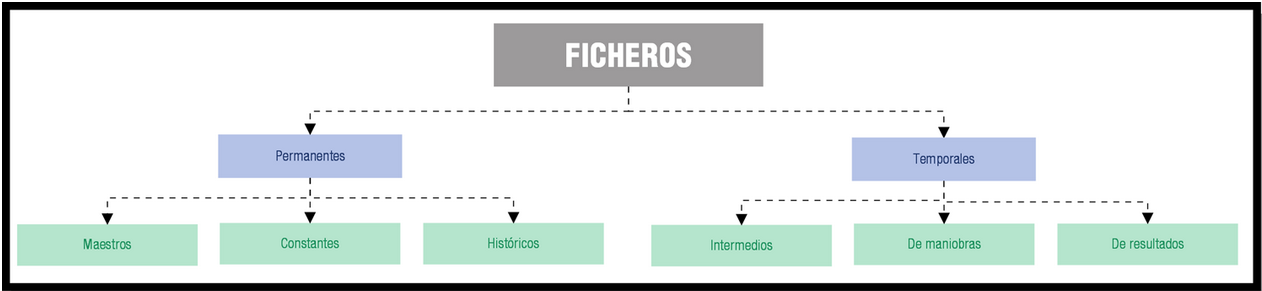
\includegraphics[scale=0.35]{ficheros-tipos.png}
    \caption{Clasificación de ficheros según su función}
\end{figure}

\subsection{Los Soportes de la Información}
Los ficheros se almacenan en soportes de información manejados por periféricos del ordenador, que permiten leer y grabar datos en el soporte. Los soportes más utilizados son las \textbf{cintas magnéticas} y los \textbf{discos} (magnéticos, ópticos o magneto-ópticos).

Al principio se usaban tambores de cinta magnética, similares en tamaño a un disco de vinilo, funcionaban de manera similar a los antiguos casetes, pero al tener un tamaño mucho más grande permitían almacenar mucha mas información, permitiendo el acceso a esta de forma secuencia.

Posteriormente los medios de almacenamiento fueron evolucionando a la par que el hardware, en concreto con la aparición de los disquetes y el disco duro. Estos dispositivos ya permitían el acceso aleatorio a los datos.

Por lo tanto, podemos distinguir dos tipos de dispositivos de almacenamiento de datos:

\begin{itemize}
    \item \textbf{Soportes de Acceso Directo a Datos}: son los más empleados y el acceso a datos se hacer de forma directa, pudiendo colocarlos en la posición que más nos interese.
    \item \textbf{Soporte de Acceso Secuencial}: se suele usar en copias de seguridad y si deseamos leer un dato que esta a mitad de la cinta, tendremos que leer todo lo que hay hasta llegar a esa posición.
\end{itemize}

Si quieres aprender más sobre las características de cintas y discos, puedes consultar los enlaces siguientes:

\begin{itemize}
    \item \href{https://es.wikipedia.org/wiki/Cinta_magn\%C3\%A9tica_de_almacenamiento_de_datos}{Cintas magnéticas de almacenamiento de datos}
    \item \href{https://es.wikipedia.org/wiki/Disco_magn\%C3\%A9tico}{Discos magnéticos} y \href{https://es.wikipedia.org/wiki/Disco_\%C3\%B3ptico}{Discos ópticos}
\end{itemize}

\subsection{Métodos de Acceso a Ficheros}
A medida que la tecnología ha ido evolucionando, el acceso a la información ha ido variando mucho. Los objetivos de fundamentales de estas variaciones son los siguientes:

\begin{itemize}
    \item Proporcionar acceso rápido a los registros.
    \item Conseguir economizar el almacenamiento.
    \item Facilitar la actualización de los registros.
    \item Permitir que la estructura refleje la organización real de la información.
\end{itemize}

Los ficheros se pueden clasificar según como se organiza en la memoria principal, o dicho de otra forma, los métodos de acceso al fichero, que podemos ver en la siguiente figura.

\begin{figure}[ht]
    \centering
    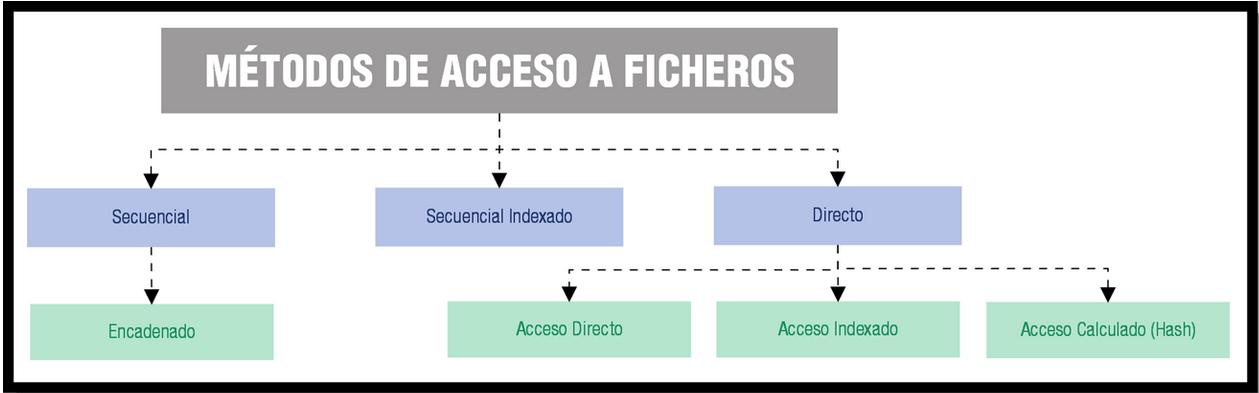
\includegraphics[scale=0.40]{ficheros-acceso.png}
    \caption{Tipos de ficheros por método de acceso}
\end{figure}

Las organizaciones secuencia, de acceso aleatorio o directo e indexado, son las mas comunes. En esta sección vamos a explicar las características de cada uno de los métodos de acceso a ficheros.

\subsubsection{Ficheros Secuenciales}
Un \textbf{fichero secuencial} se caracteriza porque sus registros están almacenados de forma continua, de forma que la única manera de acceder a él, es leyendo un registros detrás de otro hasta el final. En los ficheros secuenciales hay una marca que indica el final del fichero, suele denominarse \textbf{EOF} (End Of File). Así, para detectar el final de fichero solo es necesario encontrar esta marca.

Este tipo de fichero puede usar dispositivos de almacenamiento de acceso secuencial, como cintas magnéticas, aunque también se utilizan en los CD de audio y DVD de vídeo, en los que la música y las imágenes se almacenan en un espiral continua.

Los registros almacenados se identifican por medio de la información ubicada en uno de sus campos, que se denomina \textbf{clave} o \textbf{llave}. Si se ordena un archivo secuencial por su clave es más rápido realizar operaciones sobre el.

\begin{figure}[ht]
    \centering
    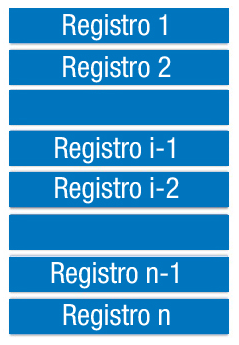
\includegraphics[scale=0.32]{fichero-secuencial.png}
    \caption{Estructura de un fichero secuencial}
\end{figure}

Algunas características de este tipo de ficheros son las siguientes:

\begin{itemize}
    \item La \textbf{lectura} siempre se realiza \textbf{hacia adelante}.
    \item Son ficheros \textbf{monousuario}, no permiten el acceso simultáneo de varios usuarios.
    \item Tiene una \textbf{estructura rígida de campos}. Todos los registros deben aparecer en orden, es decir, la posición de los campos en el registros siempre debe ser la misma.
    \item El \textbf{modo de apertura} del fichero, condiciona la lectura o escritura.
    \item \textbf{Aprovechan al máximo} el soporte de \textbf{almacenamiento}, no dejando huecos vacíos.
    \item Se pueden \textbf{grabar} en \textbf{cualquier tipo} de \textbf{soporte}, tanto secuenciales como direccionales.
    \item Todos los \textbf{lenguajes de programación} contiene instrucciones para \textbf{trabajar} con este tipo de ficheros.
    \item \textbf{No} se pueden \textbf{insertar registros} en los que están \textbf{ya grabados}.
\end{itemize}

\subsubsection{Ficheros de Acceso Directo}
En este tipo de archivos se puede acceder a un registro indicando la posición relativa del registros dentro del archivo, o a través de una \textbf{clave} que forma parte del registro como un \textbf{campo} más. Estos archivos deben almacenarse en dispositivos de memoria masiva con acceso directo como los discos magnéticos.

Cada uno de los registros se guarda en una posición física, que dependerá del espacio disponible en memoria masiva, por lo que la distribución es aleatoria dentro del soporte de almacenamiento. Para acceder a la posición física del registros se utiliza una posición o índice, de forma que no es necesario recorrer todo el fichero para encontrar un determinado registros.

 Esta \textbf{dirección física} se obtendrá tras la aplicación de una \textbf{transformación} específica a la \textbf{clave}. Según como sea esta transformación, existen tres modos de acceso diferente, como podemos ver en la siguiente figura.

\begin{figure}[ht]
     \centering
     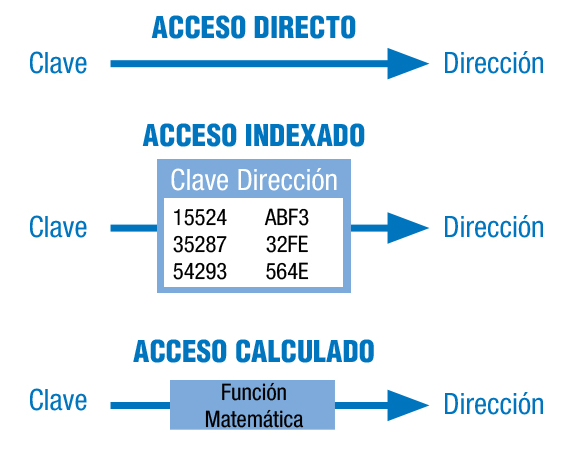
\includegraphics[scale=0.32]{fichero-accesodirecto.png}
     \caption{Modos de acceso a un registro en archivos de acceso directo}
 \end{figure}

El método más rápidos es el \textbf{acceso directo}, donde la clave coincide con la dirección física del registro, teniendo ésta que ser una posición valida dentro del rango de direcciones físicas.

La \textbf{medida de posicionamiento} básico del puntero en el fichero es el \textbf{byte}, dependiendo del tipo de codificación de caracteres que empleemos (\textbf{\gls{Unicode}}, \textbf{\gls{ANSI}}), se usarán 1 o 2 bytes por carácter respectivamente. Teniendo esto en cuenta, el puntero avanza de 1 en 1 o de 2 en 2 bytes para poder leer o escribir cada carácter.

Otras \textbf{características} de este tipo de ficheros son las siguientes:

\begin{itemize}
    \item \textbf{Posicionamiento inmediato}.
    \item \textbf{Registros} de \textbf{longitud fija}.
    \item \textbf{Apertura} del fichero en \textbf{modo mixto}, para lectura y escritura.
    \item Permiten \textbf{múltiples usuarios} al mismo tiempo.
    \item Los \textbf{registros se borran} colocando un cero en la posición que ocupan.
    \item Permiten la utilización de \textbf{algoritmos de compactación} de huecos.
    \item Los archivos se \textbf{crean} con un \textbf{tamaño definido}, es decir, con un máximo de registros definidos durante su creación.
    \item Esta organización solo es posible en \textbf{soportes direccionales}.
    \item Se \textbf{usan} cuando el \textbf{acceso a datos} de un registro se hace siempre empleando la \textbf{misma clave} y la \textbf{velocidad de acceso} al registro es lo que más importa.
    \item Permiten la \textbf{actualización de registros} en el mismo fichero, sin necesidad de copiarlo.
    \item Permiten realizar \textbf{procesos de actualización} en \textbf{tiempo real}.
\end{itemize}

\subsubsection{Ficheros Indexados}
Se basan en el uso de \textbf{indices}, que permiten el acceso a un registros sin tener leer el fichero entero. Estos indices son similares a los de los libros, si nos interesa leer un capítulo podemos recurrir al indice donde se nos dice en que página comienza y acaba dicho capítulo.

Por lo tanto, deberá existir una \textbf{zona de registros} en los que se encuentren los datos del archivo y una \textbf{zona de índices}, que contiene la tabla con las claves de los registros y las posiciones donde se encuentran. La tabla de índices esta ordenada por campos clave.

La tabla de índices será cargada en la memoria principal para realizar en ella la búsqueda de la fila correspondiente a la clave del registros a encontrar, proporcionando así la dirección donde se encuentra el registro. Una vez localizada la dirección, solo es necesario acceder el dispositivo de almacenamiento y colocarlos en la dirección indicada.

\begin{figure}[ht]
    \centering
    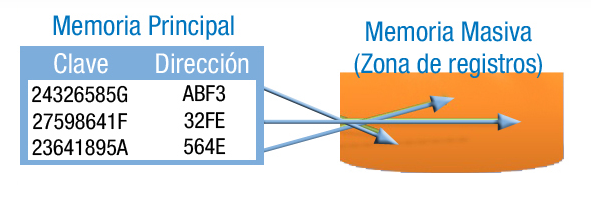
\includegraphics[scale=0.50]{fichero-indexado.png}
    \caption{Ficheros indexados}
\end{figure}

Las características mas relevantes de los ficheros indexados son las siguientes:
\begin{itemize}
    \item El diseño de registros tiene que tener un campo o campos, que permita identificar cada registro de forma única, es decir, no puede haber 2 registros que tengan la misma información en él. A este campo se le llama \textbf{campo clave} y es el que va a servir de índice. Un mismo fichero puede tener varios campos clave, pero al menos uno de ellos \textbf{no puede tener valores duplicados} y se llama \textbf{clave principal}. A las restantes se les llama \textbf{claves alternativas}.
    \item Permite usar el modo de \textbf{acceso secuencial} y el modo de \textbf{acceso directo} para leer la información que guardan sus registros.
    \item Para acceder a estos ficheros usando el modo de \textbf{acceso directo}, se hace conociendo el \textbf{contenido} del \textbf{campo clave} que queremos localizar. Con esta información el sistema operativo puede consultar el índice y conocer la posición dentro del fichero.
    \item Para acceder a este tipo de ficheros usando el m\textbf{modo secuencial}, los registros son \textbf{leídos} por el contenido del \textbf{campo clave}, independientemente del orden en el que fueron grabados, ya que el acceso se hace a través del índice, que para hacer más fácil la búsqueda de registros, permanece siempre ordenado por campos clave.
    \item Solamente puede \textbf{almacenarse} en un \textbf{medio direccionable}, ya que sino no podría usar el modo de acceso directo.
\end{itemize}

\subsubsection{Otros Tipos de Organización}
Además de los tipos de organización de ficheros que ya hemos visto, existen otros como los \textbf{ficheros secuenciales indexados} o los \textbf{ficheros de acceso calculado}, los cuales pasamos a describir a continuación.

\begin{enumerate}[label=(\alph*)]
    \item \textbf{Ficheros Secuenciales Indexados}:

    También llamados parcialmente indexados, al igual que los ficheros indexados existe una \textbf{zona de índices} y otra \textbf{zona de registros de datos}, pero esta última se encuentra \textbf{dividida} en \textbf{segmentos} ordenados.

    En la zona de índices, cada fila hace referencia a cada uno de los segmento. La clave corresponde al último registros del segmento y el índice al registro inicial. Una vez que se accede al primer registro del segmento, dentro de él se localiza (de forma secuencial) el registro buscado.

    Las principales características de este tipo de ficheros son:
    \begin{itemize}
        \item Permite el \textbf{acceso secuencial}. Esto es muy interesante cuando la tasa de accesos es alta. En el acceso secuencial ademas los registros se leen ordenados por el campo clave.
        \item Permite el \textbf{acceso directo a registros}. Realmente \textbf{emula} este tipo de acceso, empleando para ello las tablas de índices. Primero busca la clave en el área de índices y luego va a leer al área de datos en al dirección que indica la tabla.
        \item Se pueden \textbf{actualizar} los \textbf{registros} en el \textbf{mismo fichero}, sin necesidad de crear uno nuevo de copia en el proceso de actualización.
        \item Ocupa \textbf{más espacio} que los \textbf{ficheros secuenciales}, debido al uso del área de índices.
        \item Solo se pueden utilizar \textbf{soportes direccionales}.
        \item Obliga a una \textbf{inversión económica mayor}, por la necesidad de \textbf{programas}, y a veces, \textbf{hardware más sofisticado}.
    \end{itemize}

    \item \textbf{Ficheros de Acceso Calculado o Hash}:

    Cuando usamos ficheros indexados es necesario siempre consultar una tabla para obtener la dirección de almacenamiento a partir de la clave. La técnica de acceso calculado o \textbf{hash}, permite accesos más rápidos, ya que en vez de consultar una tabla utiliza una \textbf{función matemática} (función de hashing) conocida, que a partir de la clave genera la dirección conocida de cada registro. Si la clave el alfanumérica deberá previamente ser transformada en un número.

    El mayor problema que ofrece esta aproximación es que a partir de diferentes claves se puedan obtener la misma dirección de almacenamiento al aplicar la función. A este problema se le denomina \textbf{colisión}, y las claves que generan la misma dirección se denominan \textbf{sinónimos}. Para resolver este problema se aplican diferentes métodos, como tener un bloque de excedentes o zona de sinónimos, o crear un archivo de sinónimos, etc...

    Para llevar a cabo la transformación se existen multitud de métodos, aunque los mas empleados son:

    \begin{itemize}
        \item \textbf{Módulo}: la dirección será igual al resto de la división entera entre la clave y el número de registros.
        \item \textbf{Extracción}: la dirección será igual a una parte de las cifras que se extraen de la clave.
    \end{itemize}

    Una buena función hash, será aquella que produzca el menor número de colisiones. En este caso hay que buscar una función, a poder ser \textbf{\gls{biunivoca}}, que relaciones los posibles valores de la clave con el conjunto de números correlativos de la dirección. Esta función consistirá en realizar una serie de cálculos matemáticos con el valor de la clave hasta obtener un número entre 1 y n, siendo n el número de direcciones que tiene el fichero.
\end{enumerate}

\subsection{Parámetros de Utilización}
En función del uso que se le vaya a dar al fichero, serán convenientes unos u otros métodos de organización. Mediante la utilización de \textbf{parámetros de referencia} podemos determinar el uso de un fichero. Estos parámetros son:

\begin{enumerate}[label=(\alph*)]
    \item \textbf{Capacidad o Volumen}: es el espacio, en caracteres, que ocupa el fichero. La capacidad podrá calcularse multiplicando el número de registros por el tamaño medio de cada registro.
    \item \textbf{Actividad}: permite conocer la cantidad de consultar y modificaciones que se realizan en un fichero. Para poder especificar la actividad hay que tener en cuenta:
    \begin{itemize}
        \item \textbf{Tasa de Consulta o Modificación}: que es el número de registros consultar o modificados en cada tratamiento del fichero, respecto al número total de registros contenidos en él.
        \item \textbf{Frecuencia de Consulta o Modificación}: número de veces que se accede a un fichero para realizar una consulta o modificación en un tiempo predeterminado.
    \end{itemize}

    \textbf{Volatilidad}: mide la cantidad de inserciones y borrados que se efectúan en un fichero. Para determinar la volatilidad es necesario saber:
    \begin{itemize}
        \item \textbf{Tasa de Renovación}: es el tanto por ciento de registros renovados en cada tratamiento del fichero respecto del número de registros totales.
        \item \textbf{Frecuencia de Renovación}: es el número de veces que se accede al fichero para renovarlo durante un período de tiempo determinado.
    \end{itemize}

    \item \textbf{Crecimiento}: es la variación de la capacidad del fichero y se mide con la tasa de crecimiento, que es el porcentaje de registros en los que aumenta el fichero en cada tratamiento.
\end{enumerate}

Teniendo en cuenta estos valores, podremos hacernos una idea de cual es el método de organización que mejor se adapta a nuestra necesidades y cual es el que deberemos usar en nuestros ficheros.

\newpage

\section{Bases de Datos}
Como hemos visto en la sección anterior, los fichero permiten organizar y memorizar conjuntos de datos de un mismo tipo con una determinada estructura, siendo un medio para almacenar la información o resultados de una aplicación. El problema es que si las aplicaciones, al ser diseñadas, dependen directamente de sus archivos, se pierde independencia y surgen serios inconvenientes: como información duplicada, incoherencia de datos, etc...

Aquí es donde aparece el concepto de base de datos. Una \textbf{base de datos} permitirá reunir toda la información relacionada en un único sistema de almacenamiento, pudiendo cualquier aplicación utilizarla de forma independiente y ofreciendo una mejora en el tratamiento de la información.

La gestión de las bases de datos a experimentado gran cantidad de cambios, partiendo de aplicaciones especializadas hasta pasar a convertirse en el núcleo de los entornos informáticos modernos. Con la llegada de internet en los 90, el número de usuario de bases de datos creció exponencialmente, y aunque muchos no sean conscientes de ello, las usan a diario.

Así, conocer los sistemas de gestión de bases de datos, sus conceptos fundamentales, el diseño, lenguajes e implementación de estas, es imprescindible para cualquiera que se este formando en el campo de la informática.

\subsection{Conceptos Básicos}
Una \textbf{base de datos} es una colección de datos relacionados lógicamente entre sí, con una definición y descripción comunes y que están estructurados de una determinada manera. Es un conjunto de datos que representa entidades y sus relaciones, almacenados con la mínima redundancia y posibilitando el acceso a ellos eficientemente por parte de varias aplicaciones.

Las bases de datos no contienen solo los datos de la organización, sino que también almacenan una descripción de dichos datos. Esta descripción es lo que se denomina \textbf{metadatos}, se almacenan en un \textbf{diccionario de datos} o \textbf{catálogo} y es lo que permite la \textbf{independencia de datos} lógico-física.

Una base de datos, constará de los siguientes \textbf{elementos}:
\begin{itemize}
    \item \textbf{Entidades}: objeto real o abstracto, con características diferenciadas de otros, del que se almacena información en la base de datos. En una base de datos de una clínica veterinaria, diferentes entidades podrían ser: ejemplar, doctor, consulta, etc...
    \item \textbf{Atributos}: son los datos que se almacenan en la entidad. Cualquier propiedad o característica puede ser un atributo de una entidad. Continuando con el ejemplo, podrían ser atributos: raza, color, nombre, número de identificación, etc...
    \item \textbf{Registros}: es donde se almacena la información de cada entidad. Es un conjunto de atributos que contienen los datos que pertenecen a una misma repetición de identidad. En nuestro ejemplo un registros podría ser: Podenco, blanco, 121932911, etc...
    \item \textbf{Campos}: donde se almacenan los atributos de cada registro. Teniendo en cuento el ejemplo anterior, un campo podría ser Podenco.
\end{itemize}

El uso de bases de datos ofrece muchas \textbf{ventajas}, entre las que podemos encontrar las siguientes:

\begin{itemize}
    \item \textbf{Acceso Múltiple}: diversos usuarios y aplicaciones podrán acceder a la base de datos sin que existan problemas en el acceso o los datos.
    \item \textbf{Utilización Múltiple}: cada uno de los usuarios o aplicaciones podrá tener una visión única de la base de la estructura de la base de datos, accediendo solo a la parte que le corresponde.
    \item \textbf{Flexibilidad}: la forma de acceso de la información puede ser establecida de diferentes maneras, ofreciendo tiempos de respuesta muy reducidos.
    \item \textbf{Confidencialidad y Seguridad}: el control de acceso de los datos podrá ser establecido para que los usuarios y aplicaciones puedan acceder a unos datos y a otros no, impidiendo a los usuarios no autorizados el uso de la base de datos.
    \item \textbf{Protección Contra Fallos}: en casos de fallos en la información, existen mecanismos bien definidos que permiten la recuperación de los datos de forma fiable.
    \item \textbf{Independencia Física}: un cambio en el soporte físico, por ejemplo un disco duro, no afectaría a los datos o las aplicaciones que acceden a estos.
    \item \textbf{Independencia Lógica}: los datos realizados en la base de datos no afectan a las aplicaciones que acceden a ella.
    \item \textbf{Redundancia}: los datos se almacenan, por lo general, una única vez, aunque si fuera necesario podríamos repetir la información de manera controlada.
    \item \textbf{Interfaz de Alto Nivel}: mediante la utilización de lenguajes de alto nivel puede utilizarse la base de datos de forma sencilla y cómoda.
    \item \textbf{Consulta Directa}: existe una herramienta para poder acceder a los datos de forma interactiva.
\end{itemize}

\subsection{Uso de las Bases de Datos}
Ya sabemos en que consiste una base de datos, ahora veremos que usuarios son los que la utilizan y en que campos se utilizan éstas.

Existen principalmente cuatro \textbf{tipos de personas} que pueden hacer uso de las bases de datos y cada uno de ellos hace un uso diferente de éstas. Estas personas son:

\begin{itemize}
    \item \textbf{El Administrador}

    Es la persona encargada de la creación o implementación física de la base de datos. Es quien escoge los tipos de ficheros, los índices que se deben crear, la ubicación de estos, etc... En general, es quien toma las decisiones del funcionamiento físico del almacenamiento de la información. Además, establecerá la política de seguridad y acceso para garantizar el menos número de problemas.

    \item \textbf{Los Diseñadores}

    Son los encargados de diseñar como será la base de datos. Llevarán a cabo la identificación de los datos, sus relaciones, sus restricciones, etc... Para ello, han de conocer a fondo los datos y procesos que deben representarse en la base de datos. Si estamos hablando de una empresa, deberán conocer la reglas de negocio de esta. Para obtener un buen resultado, el diseñador deberá implicar a todos los usuarios de la base de datos lo antes posible en el proceso.

    \item \textbf{Los Programadores de Aplicaciones}

    Una vez diseñada y construida la base de datos, los programadores se encargarán de implementar los programas de aplicación que servirán a los usuarios finales. Estos programas permitirán la posibilidad de realizar inserciones, actualizaciones o eliminaciones de datos. Para desarrollar estas aplicaciones se utilizan lenguajes de tercera o cuarta generación, como C, FORTRAN, Smalltalk, Ada, Java, etc...

    \newpage

    \item \textbf{Los Usuarios Finales}

    Son los clientes finales de la base de datos. Al diseñar, implementar y mantener la base de datos se busca cumplir con los requisitos establecidos por el cliente para la gestión de su información.
\end{itemize}


Respecto a los \textbf{campos} en los que se\textbf{ usan la bases de datos} y los usos que se les dan son innumerables, aunque en la siguiente lista tienes algunos ejemplos:

\begin{itemize}
    \item Banca: información de clientes, cuentas, transacciones, ...
    \item Líneas Aéreas: información de clientes, vuelos, horarios, ...
    \item Universidades: información de alumnos, asignaturas, profesores, horarios,...
    \item Telecomunicaciones: guardar registros de llamadas realizadas, generar facturas mensuales, mantener saldo de las tarjetas telefónicas y almacenar información sobre las redes.
    \item Medicina: información hospitalaria, biomedicina, genética, ...
    \item Legislación: normativas, registros, etc...
    \item Organismos Públicos: registros de los ciudadanos, certificados, etc...
    \item Justicia y Seguridad: delincuentes, casos, sentencias, investigaciones...
\end{itemize}

Como vemos, prácticamente en cualquier campo en el que se necesite recopilar, almacenar y gestionar información se utilizan las bases de datos.

\subsection{Ubicación de la Información}
Las bases de datos pueden tener un tamaño muy pequeño o ser muy voluminosas, pero independientemente de esto todas se almacenan en discos duros y otros dispositivos de almacenamiento a los que se puede acceder a través de un ordenador. Una base de datos pequeña pueden existir en un archivo pequeño dentro de un disco duro, mientras que una gran base de datos puede necesitar decenas de servidores en diferentes localizaciones.

En esta sección, vamos a ver los tipos de dispositivos y tecnologías de almacenamiento mas utilizados para el despliegue de bases de datos. En la siguiente lista, se detallan estos dispositivos:

\begin{itemize}
    \item \item \textbf{Disco SATA}: es una interfaz de transferencia de datos entre la placa base y algunos dispositivos de almacenamiento como discos duros, lectores o grabadores de CD/DVD, unidades de estado solido u otros dispositivos. La interfaz SATA proporciona mayores velocidades, cables de conexión mas largos, mejor aprovechamiento cuando hay varios dispositivos conectados y capacidad de conectar unidades sin necesidad de apagar el ordenador. La primera generación tenía una tasa de transferencia de 150 MB/s, denominada \textbf{SATA 150 MB/s} o \textbf{Serial-ATA-150}. Actualmente se comercializan dispositivos \textbf{SATA II}, con velocidades de transferencia de 300 MB/s y \textbf{SATA III}, con velocidades de 600 MB/s.

    \item \textbf{Discos SCSI}: son interfaces preparadas para discos de gran capacidad de almacenamiento y gran velocidad de rotación. Se presentan bajo tres especificaciones: \textbf{Standard SCSI}, \textbf{Fast SCSI} y \textbf{Fast-Wide SCSI}. Su velocidad de acceso puede llegar a los 7 ms y la velocidad de transmisión de información secuencia a 5 MB/s, 10 MB/s y 20 MB/s para las versiones Standard, Fast y Fast-Wide respectivamente. Un controlador puede manejar hasta 7 discos duros SCSI.

    \item \textbf{RAID}: acronimo de \textbf{Redundant Array of Independent Disks}, es un contenedor de almacenamiento redundante. Se basa en montar varios discos duros para que trabajen conjuntamente obteniendo mejoras en el almacenamiento, la velocidad, la disponibilidad y la seguridad de la información. Según las características que queramos reforzar se usará una u otra configuración RAID.

    \item \textbf{Sistemas NAS}: es el acrónimo de \textbf{Network Attached Storage}. Estos sistemas de almacenamiento permiten compartir el almacenamiento de un computador (servidor), con ordenadores personales o servidores clientes a través de la red, haciendo uso de un sistema operativo optimizado para dar acceso a los datos a través de protocolos de comunicación específicos. Suelen ser dispositivos de almacenamiento de gran capacidad, varios TeraBytes, generalmente superiores a los discos duros externos y que están conectados con la red.

    \item \textbf{SAN}: acrónimo de \textbf{Storage Area Network}. Se trata de una red concebida, arrays de discos y librerías de soporte. La arquitectura de este tipo de sistema permite que los recursos de almacenamiento estén disponibles para varios servidores en una red de área local o amplia. Debido a que la información almacenada no reside en directamente en ninguno de los equipos de la red, se optimiza el poder de procesamiento para aplicaciones comerciales y la capacidad de almacenamiento se puede proporcionar al servidor que más lo necesite.
\end{itemize}

Aunque no se mencionen en esta lista, en los últimos años la tendencia es usar \textbf{bases de datos en la nube}, que permiten la utilización de bases de datos desarrolladas, implementadas y a las que se accede en un entorno de nube, como una nube privada, pública o híbrida. \cite{cloud01} En la \href{https://www.oracle.com/es/database/what-is-a-cloud-database/}{página de Oracle} puedes encontrar información más detallada sobre este tipo de bases de datos.

\section{Modelos de Bases de Datos}
La clasificación tradicional de las bases de datos establece tres modelos de bases de datos: \textbf{jerárquico}, \textbf{en red} y \textbf{relacional}. En la actualidad el modelo de datos mas empleado es el relacional, aunque hay que tener en cuenta que dos de sus variantes, \textbf{bases de datos distribuidas} y \textbf{orientadas a objetos} son las más empleadas.

En esta sección, vamos a analizar estos modelos de bases de datos así como algunos otros aquí no mencionados.

\subsection{Modelo Jerárquico}
Cuando IBM creó su Sistema Administrado de la Información o IMS, se establecieron las bases para que la gran mayoría de sistemas de gestión de información de los años 70 utilizaran un modelo jerárquico. También recibe el nombre de modelo árbol, ya que utiliza una estructura de árbol invertido para el almacenamiento de los datos.

En el \textbf{modelo jerárquico}, la información se organiza con un jerarquía en el que se establece una relación entre las entidades \textbf{padre/hijo}. De tal forma que existen nodos que contienen atributos o campos y que se relacionan con sus nodos hijos, pudiendo tener cada nodo \textbf{varios hijos}, pero un nodo solo puede tener \textbf{un nodo padre}.

Los \textbf{datos} de este modelo se \textbf{almacenan} en estructuras lógicas llamadas \textbf{segmentos}. Los segmentos se relacionan entre sí usando \textbf{arcos}. Visualmente, este modelo se puede representar como un árbol invertido, estando en la parte superior los padres y en la inferior los hijos.

Hoy en día, debido a sus limitaciones, este modelo esta en desuso. En la siguiente figura podemos ver un ejemplo de estructura jerárquica.

\begin{figure}[ht]
    \centering
    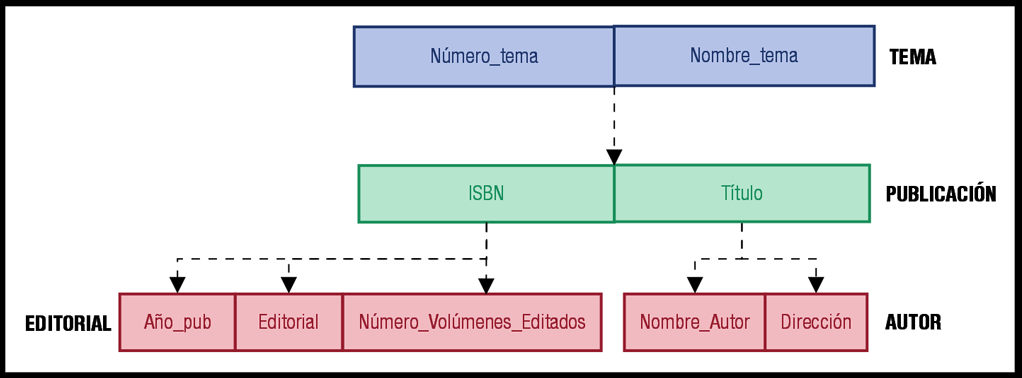
\includegraphics[scale=0.40]{bd-jerarquico.png}
    \caption{Modelo Jerárquico de Bases de Datos}
\end{figure}

\subsection{Modelo en Red}
El modelo de datos en red aparece a mediados de los 60 como respuesta a las limitaciones del modelo jerárquico en cuanto a la representación de relaciones más complejas. Podemos considerar a \textbf{IDS} (Integrated Data Storage) de Bachman como el primer sistema de bases de datos en red. Más adelante, se intento crear un modelo de red por parte de \textbf{\gls{CODASY}}, siendo un modelo que tuvo un gran aceptación a principios de los 70.

El \textbf{modelo en red} organiza la información en \textbf{registros}, también llamados nodos, y \textbf{enlaces}. En los registros se almacenan los datos, mientras que los enlaces permiten relacionar los datos. Las bases de datos en red son parecidas a las jerárquicas, salvo que en éstas un nodo puede tener \textbf{más de un padre}.

En este modelo se puede representar prácticamente cualquier relación de datos, pero su manejo se hace muy complicado. Al no tener que duplicar la información  se ahora en espacio de almacenamiento. El sistema de gestión de la información mas extendido es \textbf{\gls{IDMS}}.

En la siguiente figura podemos ver un ejemplo de este tipo de modelo de bases de datos.

\begin{figure}[ht]
    \centering
    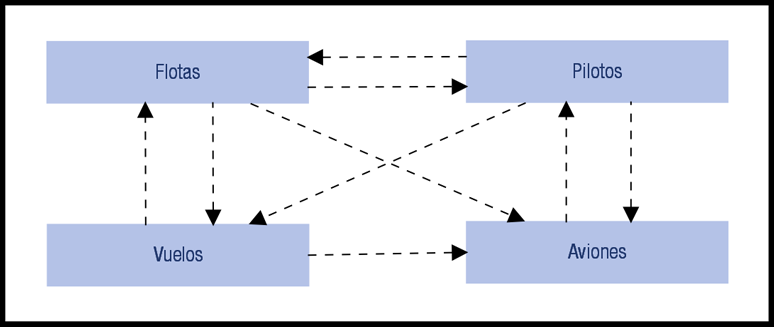
\includegraphics[scale=0.55]{bd-enred.png}
    \caption{Modelo en Red de Bases de Datos}
\end{figure}

\subsection{Modelo Relacional}
Este modelo es posterior a los dos anteriores y fue desarrollado por Codd en 1970. Hoy en día, este tipo de base de datos es la más utilizada.

El \textbf{modelo relacional} es percibida por los usuarios como un conjunto de tablas. Esta percepción es solo a nivel lógico, ya que a nivel físico puede estar implementada mediante diferentes estructuras de almacenamiento. Es modelo utiliza \textbf{tablas bidimensionales} (relaciones) para la representación lógica de los datos y las relaciones entre ellos. Cada relación (tabla) posee un nombre único y contiene un conjunto de columnas.

Cada tabla estará compuesta de los siguientes elementos:

\begin{itemize}
    \item \textbf{Registro/Entidad/Tupla}: es el nombre que recibe cada fila.
    \item \textbf{Campo/Atributo}: es el nombre que recibe cada columna.
    \item \textbf{Clave}: es el atributo o conjunto de estos que identifica de forma única a cada tupla.
\end{itemize}

Al conjunto de valores que puede tomar un atributo se le conoce como \textbf{dominio}. Ademas, las tablas deben cumplir un conjunto de \textbf{requisitos} para que se consideren correctas, que son los siguientes:

\begin{itemize}
    \item Todos los registros son del mismo tipo
    \item La tabla solo puede tener un tipo de registro.
    \item No existen campos o atributos repetidos.
    \item No existen registros duplicados.
    \item No existe orden de almacenamiento de los registros.
    \item Cada registro o tupla debe estar identificada por una clave formada por uno o varios atributos.
\end{itemize}

En la siguiente imagen puedes ver como se relacionan las tuplas y atributos en una base de datos con el modelo relacional.

    \begin{figure}[ht]
    \centering
    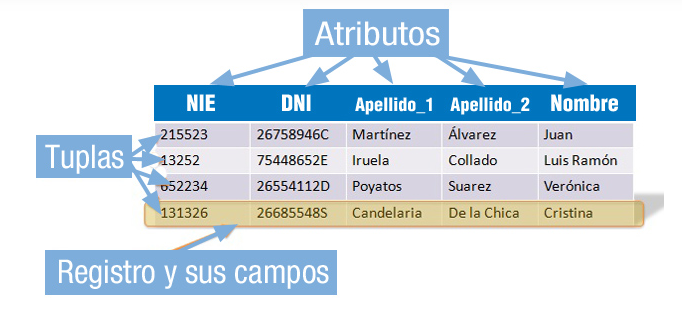
\includegraphics[scale=0.55]{bd-relacional.png}
    \caption{Modelo Relacional de Bases de Datos}
\end{figure}

El lenguaje mas habitual para construir consultas en este tipo de bases de datos es \textbf{SQL} (Structured Query Language), un estándar implementado por los principales motores o sistemas de gestión de bases de datos.

Durante su diseño, una base de datos relacional para por un proceso que se conoce como \textbf{normalización}, que consiste en definir las reglas que determinan las dependencias entre los datos. Si definimos esta dependencia en una base de datos de la forma mas sencilla posible, conseguiremos que la cantidad de espacio necesaria para almacenar los datos sea la menor posible y la facilidad para actualizar la relación sea la mayor posible. Es decir, optimizaremos su funcionamiento.

\subsection{Modelo Orientado a Objetos}
El \textbf{modelo orientado a objetos} define una base de datos en términos de \textbf{objetos}, sus \textbf{propiedades} y sus \textbf{operaciones}. Los objetos con las misma estructura y comportamiento pertenecen a una misma \textbf{clase}, y las clases se organizan en jerarquías. Las operaciones de cada clase se especifican en términos de procedimientos predefinidos denominados \textbf{métodos}. Algunos sistemas existentes en el mercado, basados en el modelo relacional, han sufrido evoluciones incorporando conceptos de la programación orientada a objetos. A estos modelos se les conoce como \textbf{modelos objeto-relacionales}.

El objetivo de este modelo es cubrir las limitaciones del modelo relacional. Gracias a este modelo se incorporan ventajas como la herencia entre tablas, los tipos definidos por el usuario, disparadores almacenables en la base de datos (triggers), soporte multimedia, etc..

En la siguiente imagen, podemos ver un ejemplo del modelo orientado a objetos.

\begin{figure}[ht]
    \centering
    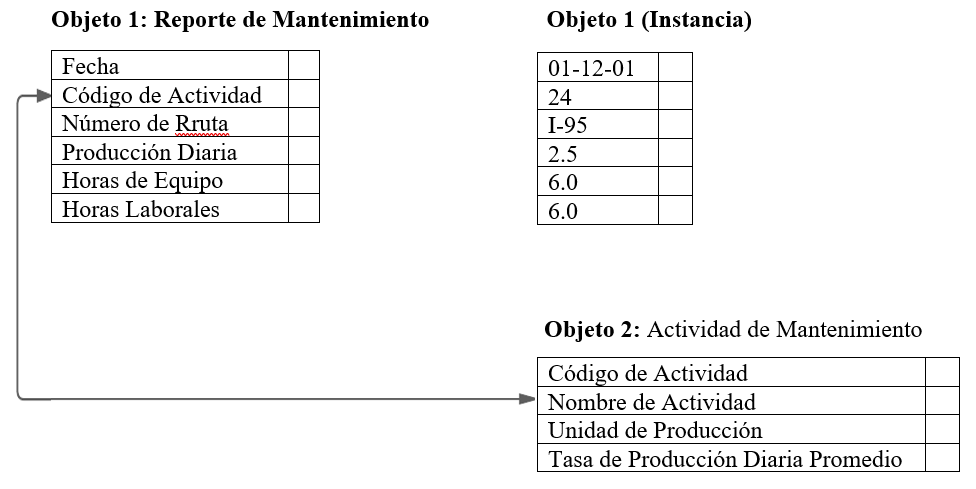
\includegraphics[scale=0.40]{bd-oo.png}
    \caption{Modelo Orientado a Objetos de Bases de Datos}
\end{figure}

Los conceptos más importantes del paradigma de objetos que incorpora el modelo orientado a objetos son los siguientes:

\begin{itemize}
    \item \textbf{Encapsulación}: propiedad que permite ocultar la información al resto de objetos impidiendo así el acceso incorrecto o conflictos.
    \item \textbf{Herencia}: propiedad a través de la cual objetos heredan comportamientos dentro de la jerarquía de clases.
    \item \textbf{Polimorfismo}: propiedad de una operación mediante la cual puede ser aplicada a diferentes tipos de objetos.
\end{itemize}

Desde la aparición de la programación orientados a objetos (OOP) se empezó a pensar en bases de datos adaptadas a estos lenguajes. Este modelo es considerado como el fundamento de las bases de datos de tercera generación, siendo considerara las bases de datos en red como la primera y las relacionales como la segunda generación. Aunque no ha reemplazado a estas últimas, si es el tipo de base de datos que más esta creciendo en los últimos años.

\subsection{Modelo NoSQL}
Las \textbf{bases de datos NoSQL} son bases de datos que no cumplen con el esquema entidad-relación. Tampoco utilizan una estructura de datos de datos en forma de tabla donde se van almacenando los datos, sino que el para el almacenamiento se usan otros formatos como clave-valor, mapeo de columnas, graos, etc...

Esta forma de almacenar los datos tiene ciertas \textbf{ventajas} respecto a los modelos relacionales, las cuales son las siguientes:

\begin{itemize}
    \item Se pueden \textbf{ejecutar} en máquinas con \textbf{pocos recursos}, no requieren apenas computación.
    \item \textbf{Escalabilidad horizontal}: para mejorar el rendimiento de estos sistemas simplemente se consigue añadiendo mas nodos, con la única operación de indicar al sistema cuales son los nodos que están disponibles.
    \item Puede manejar \textbf{gran cantidad de datos}, debido a que usan una \textbf{estructura distribuida} en muchos casos mediante \textbf{tablas Hash}.
    \item \textbf{No generan cuellos de botella}: el principal problema de los sistema SQL es que necesitan transcribir cada sentencia para poder ser ejecutada, lo que constituye a un punto de entrada común, que ante muchas peticiones puede ralentizar el sistema.
\end{itemize}

Después de ver las principales ventajas que tiene el uso de este modelo, en la siguiente lista vemos las principales \textbf{diferencias} que nos podemos encontrar entre las bases de datos \textbf{NoSQL} y los sistemas \textbf{SQL} son las siguientes:

\begin{itemize}
    \item \textbf{No utilizan SQL} como lenguaje de consulta. La mayoría de bases de datos NoSQL evitan usar este lenguaje o, como mucho, lo usan como apoyo.
    \item \textbf{No utilizan} estructuras fijas como \textbf{tablas} para el almacenamiento de datos. Permiten hacer uso de otros sistemas de almacenamiento de información como clave-valor, objetos o grafos.
    \item \textbf{No} suelen permitir \textbf{operaciones JOIN}. Al disponer de un volumen de datos tan extremadamente grande cuando la operación no es la búsqueda de una clave, la sobrecarga puede llegar a ser muy costosa. La solución en este caso sería desnormalizar los datos, o bien realizar el JOIN mediante software en la capa de aplicación.
    \item \textbf{Arquitectura distribuida}: las bases de datos relacionales suelen estar centralizas en una misma máquina o bien en una estructura master-slave, sin embargo en los casos NoSQL la información puede estar compartida por varias máquinas mediante mecanismos de tablas Hash distribuidos.
\end{itemize}

Como hemos comentado, este modelo de bases de datos no usa tablas para almacenar datos, sino que se emplean otros tipos de almacenamiento que no suelen usar en bases de datos relacionales. Así, dependiendo del \textbf{tipo de almacenamiento} que se use en una base de datos NoSQL, estas puede pueden clasificarse en:

\begin{enumerate}[label=(\alph*)]
    \item \textbf{Bases de datos clave-valor}: es el modelo de bases de datos NoSQL más popular, además de ser el más sencillo en cuanto a funcionalidad. En este tipo de sistemas, cada elemento está identificado por una \textbf{llave única}, lo que permite la recuperación de información de una forma muy rápida. Información que habitualmente esta almacenada como un \textbf{objeto binario} (BLOB). Se caracterizan por ser \textbf{muy eficientes} tanto para las \textbf{lecturas} y las \textbf{escrituras}. Algunos ejemplos de estas bases de datos son Cassandra, BigTable o HBase.

    \item \textbf{Bases de datos documentales}: estas bases de datos almacenan la información como un documento, por norma general con una estructura simple como \textbf{JSON} o \textbf{XML} y donde se utiliza una \textbf{clave única} para cada registro. Es tipo permite, ademas de realizar búsquedas por clave-valor, realizar consultar más avanzadas sobre el contenido del documento. Son las bases de datos NoSQL \textbf{más versátiles}. Se pueden utilizar en muchos tipos de proyectos, incluso en muchos que tradicionalmente usarían bases de datos relacionales. Algunas de las mas utilizadas son MongoDB o CouchDB.

    \item \textbf{Bases de datos en grafo}: en este tipo de bases de datos, la información se presenta como nodos en un grafo y sus relaciones como aristas, de manera que se puede hacer uso de la teoría de grafos para recorrerla. Este tipo de bases de datos ofrece una navegación más eficiente que las bases de datos relacionales. Algunos ejemplos de estas bases de datos son Neo4j, InfoGrid o Virtuoso.
\end{enumerate}





% Glossary

\glsaddall
\printglossaries

% Bibliography

\newpage
\addcontentsline{toc}{chapter}{Bibliografía}
\bibliography{citas}
\bibliographystyle{unsrt}

\end{document}